\documentclass{standalone}
\usepackage{tikz}
\usepackage{ctex,siunitx}
\setCJKmainfont{Noto Serif CJK SC}
\usepackage{tkz-euclide}
\usepackage{amsmath}
\usetikzlibrary{patterns, calc,3d}
\usetikzlibrary {decorations.pathmorphing,decorations.pathreplacing,decorations.shapes,}
\begin{document}
\small
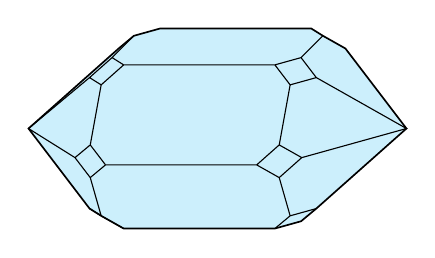
\begin{tikzpicture}[>=latex,scale=1.2]
  % \useasboundingbox(-1.0,-1.4)rectangle(3.5,3.7);
  \draw[fill=cyan!20,semithick]
  (-2.000, 0.000, 0.000)--(-1.200, 0.693,-0.400)--(-1.000, 0.866,-0.300)--(-0.800, 0.866,-0.500)--( 0.800, 0.866,-0.500)--( 1.000, 0.866,-0.300)--( 1.200, 0.693,-0.400)--( 2.000, 0.000, 0.000)--( 1.200,-0.693, 0.400)--( 1.000,-0.866, 0.300)--( 0.800,-0.866, 0.500)--(-0.800,-0.866, 0.500)--(-1.000,-0.693, 0.600)--(-1.200,-0.693, 0.400)--cycle;
  \draw[thin](-0.800,0.866,0.500)--(-1.000,0.693,0.600)--(-1.000,0.173,0.900)--(-0.800,0.000,1.000)--( 0.800,0.000,1.000)--( 1.000,0.173,0.900)--( 1.000,0.693,0.600)--( 0.800,0.866,0.500)--cycle
  (-2.000, 0.000,0.000)--(-1.200, 0.000,0.800)--(-1.000,-0.173,0.900)--(-1.000,-0.693,0.600)--(-1.200,-0.693,0.400)
(-2.000,0.000, 0.000)--(-1.200,0.693, 0.400)--(-1.000,0.866, 0.300)--(-1.000,0.866,-0.300)
(0.800,-0.866, 0.500)--(1.000,-0.693, 0.600)--(1.000,-0.173, 0.900)--(1.200, 0.000, 0.800)--(2.000, 0.000, 0.000)--(1.200, 0.693, 0.400)--(1.000, 0.866, 0.300)--(1.000, 0.866,-0.300) 
(-1.000,-0.693,0.600)--(-0.800,-0.866,0.500)
(-1.000,-0.173,0.900)--(-0.800, 0.000,1.000)
(-1.200, 0.000,0.800)--(-1.000, 0.173,0.900)
(-1.200, 0.693,0.400)--(-1.000, 0.693,0.600)
( 0.800, 0.866,0.500)--( 1.000, 0.866,0.300)
( 1.000, 0.693,0.600)--( 1.200, 0.693,0.400)
( 1.000, 0.173,0.900)--( 1.200, 0.000,0.800)
( 0.800, 0.000,1.000)--( 1.000,-0.173,0.900)
(-1.000, 0.866,0.300)--(-0.800, 0.866,0.500)
( 1.000,-0.693,0.600)--( 1.200,-0.693,0.400);
  % \draw[thin,densely dashed](1,0,0)--(0,0,-1)--(-1,0,0)(0,-1,0)--(0,0,-1)--(0,1,0);
\end{tikzpicture}
\end{document}